%% BioMed_Central_Tex_Template_v1.05
%%                                      %
%  bmc_article.tex            ver: 1.05 %
%                                       %


%%%%%%%%%%%%%%%%%%%%%%%%%%%%%%%%%%%%%%%%%
%%                                     %%
%%  LaTeX template for BioMed Central  %%
%%     journal article submissions     %%
%%                                     %%
%%         <27 January 2006>           %%
%%                                     %%
%%                                     %%
%% Uses:                               %%
%% cite.sty, url.sty, bmc_article.cls  %%
%% ifthen.sty. multicol.sty		       %%
%%									   %%
%%                                     %%
%%%%%%%%%%%%%%%%%%%%%%%%%%%%%%%%%%%%%%%%%


%%%%%%%%%%%%%%%%%%%%%%%%%%%%%%%%%%%%%%%%%%%%%%%%%%%%%%%%%%%%%%%%%%%%%
%%                                                                 %%	
%% For instructions on how to fill out this Tex template           %%
%% document please refer to Readme.pdf and the instructions for    %%
%% authors page on the biomed central website                      %%
%% http://www.biomedcentral.com/info/authors/                      %%
%%                                                                 %%
%% Please do not use \input{...} to include other tex files.       %%
%% Submit your LaTeX manuscript as one .tex document.              %%
%%                                                                 %%
%% All additional figures and files should be attached             %%
%% separately and not embedded in the \TeX\ document itself.       %%
%%                                                                 %%
%% BioMed Central currently use the MikTex distribution of         %%
%% TeX for Windows) of TeX and LaTeX.  This is available from      %%
%% http://www.miktex.org                                           %%
%%                                                                 %%
%%%%%%%%%%%%%%%%%%%%%%%%%%%%%%%%%%%%%%%%%%%%%%%%%%%%%%%%%%%%%%%%%%%%%


\NeedsTeXFormat{LaTeX2e}[1995/12/01]
\documentclass[10pt]{bmc_article}    



% Load packages
\usepackage{cite} % Make references as [1-4], not [1,2,3,4]
\usepackage{url}  % Formatting web addresses  
\usepackage{ifthen}  % Conditional 
\usepackage{multicol}   %Columns
\usepackage[utf8]{inputenc} %unicode support
%\usepackage[applemac]{inputenc} %applemac support if unicode package fails
%\usepackage[latin1]{inputenc} %UNIX support if unicode package fails
\urlstyle{rm}
 
 
%%%%%%%%%%%%%%%%%%%%%%%%%%%%%%%%%%%%%%%%%%%%%%%%%	
%%                                             %%
%%  If you wish to display your graphics for   %%
%%  your own use using includegraphic or       %%
%%  includegraphics, then comment out the      %%
%%  following two lines of code.               %%   
%%  NB: These line *must* be included when     %%
%%  submitting to BMC.                         %% 
%%  All figure files must be submitted as      %%
%%  separate graphics through the BMC          %%
%%  submission process, not included in the    %% 
%%  submitted article.                         %% 
%%                                             %%
%%%%%%%%%%%%%%%%%%%%%%%%%%%%%%%%%%%%%%%%%%%%%%%%%                     


% \def\includegraphic{}
% \def\includegraphics{}



\setlength{\topmargin}{0.0cm}
\setlength{\textheight}{21.5cm}
\setlength{\oddsidemargin}{0cm} 
\setlength{\textwidth}{16.5cm}
\setlength{\columnsep}{0.6cm}

\newboolean{publ}

%%%%%%%%%%%%%%%%%%%%%%%%%%%%%%%%%%%%%%%%%%%%%%%%%%
%%                                              %%
%% You may change the following style settings  %%
%% Should you wish to format your article       %%
%% in a publication style for printing out and  %%
%% sharing with colleagues, but ensure that     %%
%% before submitting to BMC that the style is   %%
%% returned to the Review style setting.        %%
%%                                              %%
%%%%%%%%%%%%%%%%%%%%%%%%%%%%%%%%%%%%%%%%%%%%%%%%%%
 

%Review style settings
% \newenvironment{bmcformat}{\begin{raggedright}\baselineskip20pt\sloppy\setboolean{publ}{false}}{\end{raggedright}\baselineskip20pt\sloppy}

%Publication style settings
\newenvironment{bmcformat}{\fussy\setboolean{publ}{true}}{\fussy}

% - - - - - - - - - - - - - - - - - - - - - - - - - - - - - - - - 
% User-specific packages, macros, and settings
% - - - - - - - - - - - - - - - - - - - - - - - - - - - - - - - - 
\usepackage{color} 
\usepackage{amsmath} 
% \usepackage{amsfonts} 
\usepackage{xspace}
\usepackage{bm} \bm{}
\usepackage{graphicx}
\usepackage{timestamp} 

\newcommand{\PMA}{\ensuremath{\textnormal{PM}_\textnormal{A}}\xspace}
\newcommand{\PMB}{\ensuremath{\textnormal{PM}_\textnormal{B}}\xspace}
\newcommand{\gAA}{\textnormal{AA}\xspace}
\newcommand{\gAB}{\textnormal{AB}\xspace}
\newcommand{\gBB}{\textnormal{BB}\xspace}
\newcommand{\eps}{\varepsilon\xspace}
\newcommand{\pkg}[1]{\textit{#1}\xspace}
\newcommand{\CN}{\textnormal{CN}\xspace}
\newcommand{\kb}{\textnormal{kb}\xspace}
\newcommand{\GWSSixf}{GenomeWideSNP\_6\xspace}
%\newcommand{\CP}{\ensuremath{\textnormal{CP}}\xspace}
%\newcommand{\CPs}{\ensuremath{\textnormal{CPs}}\xspace}
\newcommand{\CP}{\ensuremath{\textnormal{change point}}\xspace}
\newcommand{\CPs}{\ensuremath{\textnormal{change points}}\xspace}

\newcommand{\bx}{\mathbf{x}\xspace}
\newcommand{\by}{\mathbf{y}\xspace}
\newcommand{\bz}{\mathbf{z}\xspace}
\newcommand{\ba}{\mathbf{a}\xspace}
\newcommand{\bb}{\mathbf{b}\xspace}
\newcommand{\bA}{\mathbf{A}\xspace}
\newcommand{\bB}{\mathbf{B}\xspace}
\newcommand{\bC}{\mathbf{C}\xspace}
\newcommand{\bS}{\mathbf{S}\xspace}
\newcommand{\bU}{\mathbf{U}\xspace}
\newcommand{\bV}{\mathbf{V}\xspace}
\newcommand{\bW}{\mathbf{W}\xspace}
\newcommand{\beps}{\bm{\varepsilon}\xspace}
\newcommand{\btheta}{\bm{\theta}\xspace}
\newcommand{\bnu}{\bm{\nu}\xspace}


% Comment the 2nd row to highlight updates
% \newcommand{\updated}[2][red]{{\color{#1}{#2}}\xspace}
% \renewcommand{\updated}[2][red]{#2\xspace}

\graphicspath{{figures/col/}}

\newenvironment{TODO}{\color{red}\textbf{TODO:}}{}
\newenvironment{PN}{\color{blue}\textbf{PN:}}{}


% Begin ...
\begin{document}
\begin{bmcformat}


%%%%%%%%%%%%%%%%%%%%%%%%%%%%%%%%%%%%%%%%%%%%%%
%%                                          %%
%% Enter the title of your article here     %%
%%                                          %%
%%%%%%%%%%%%%%%%%%%%%%%%%%%%%%%%%%%%%%%%%%%%%%

\title{TumorBoost: A single-sample method for calibrating allele-specific tumor copy numbers in paired tumor-normal designs}

%%%%%%%%%%%%%%%%%%%%%%%%%%%%%%%%%%%%%%%%%%%%%%
%%                                          %%
%% Enter the authors here                   %%
%%                                          %%
%% Ensure \and is entered between all but   %%
%% the last two authors. This will be       %%
%% replaced by a comma in the final article %%
%%                                          %%
%% Ensure there are no trailing spaces at   %% 
%% the ends of the lines                    %%     	
%%                                          %%
%%%%%%%%%%%%%%%%%%%%%%%%%%%%%%%%%%%%%%%%%%%%%%


\author{Henrik Bengtsson\correspondingauthor$^1$%
       \email{Henrik Bengtsson\correspondingauthor - hb@stat.berkeley.edu}%
      \and
         Pierre Neuvial$^1$%
         \email{Pierre Neuvial -pierre@stat.berkeley.edu}
       and 
         Terence P. Speed$^{1,2}$%
         \email{Terence P. Speed - terry@stat.berkeley.edu}%
   }
      

%%%%%%%%%%%%%%%%%%%%%%%%%%%%%%%%%%%%%%%%%%%%%%
%%                                          %%
%% Enter the authors' addresses here        %%
%%                                          %%
%%%%%%%%%%%%%%%%%%%%%%%%%%%%%%%%%%%%%%%%%%%%%%

\address{%
    \iid(1) Department of Statistics, University of California, Berkeley, USA\\
    \iid(2) Bioinformatics Division, Walter \& Eliza Hall Institute of Medical Research, Parkville, Australia
}%

\maketitle

%%%%%%%%%%%%%%%%%%%%%%%%%%%%%%%%%%%%%%%%%%%%%%
%%                                          %%
%% The Abstract begins here                 %%
%%                                          %%
%% The Section headings here are those for  %%
%% a Research article submitted to a        %%
%% BMC-Series journal.                      %%  
%%                                          %%
%% If your article is not of this type,     %%
%% then refer to the Instructions for       %%
%% authors on http://www.biomedcentral.com  %%
%% and change the section headings          %%
%% accordingly.                             %%   
%%                                          %%
%%%%%%%%%%%%%%%%%%%%%%%%%%%%%%%%%%%%%%%%%%%%%%


\begin{abstract}
        % Do not use inserted blank lines (ie \\) until main body of text.
        \paragraph*{Background:} High-throughput genotyping microarrays can be used not only to assess changes in total DNA copy number but also changes in allele-specific copy numbers (ASCNs). Even after state of the art preprocessing methods, Affymetrix genotyping arrays still suffer from systematic effects that prevent them from being used effectively for downstream ASCN studies in cancers. 
      
        \paragraph*{Results:} We propose a single-sample method for calibrating ASCN estimates of a tumor based on ASCN estimates of a paired normal. The method applies to any paired tumor-normal copy number estimates regardless of technology and generation. We demonstrate that ASCNs of Affymetrix genotyping arrays have a dramatically increased signal to noise ratio after calibration.

        \paragraph*{Conclusions:} Combined with single-array preprocessing methods, such as CRMA~v2, we conclude that ASCN estimates with high precisions can be obtained from a single pair of tumor-normal hybridizations, and recommend using paired tumor-normal DNA microrarry experiments when applicable.

        \paragraph*{Availability:}
A single-sample bounded-memory implementation is available in \pkg{aroma.cn}.

\end{abstract}



\ifthenelse{\boolean{publ}}{\begin{multicols}{2}}{}




%%%%%%%%%%%%%%%%%%%%%%%%%%%%%%%%%%%%%%%%%%%%%%
%%                                          %%
%% The Main Body begins here                %%
%%                                          %%
%% The Section headings here are those for  %%
%% a Research article submitted to a        %%
%% BMC-Series journal.                      %%  
%%                                          %%
%% If your article is not of this type,     %%
%% then refer to the instructions for       %%
%% authors on:                              %%
%% http://www.biomedcentral.com/info/authors%%
%% and change the section headings          %%
%% accordingly.                             %% 
%%                                          %%
%% See the Results and Discussion section   %%
%% for details on how to create sub-sections%%
%%                                          %%
%% use \cite{...} to cite references        %%
%%  \cite{koon} and                         %%
%%  \cite{oreg,khar,zvai,xjon,schn,pond}    %%
%%  \nocite{smith,marg,hunn,advi,koha,mouse}%%
%%                                          %%
%%%%%%%%%%%%%%%%%%%%%%%%%%%%%%%%%%%%%%%%%%%%%%




%%%%%%%%%%%%%%%%
%% Background %%
%%
\section*{Background}
\label{secBackground}

\begin{itemize}
\item High-throughput genotyping microarrays for cancer studies: SNP, TCN, ASCN...
\item already several preprocessing methods out there, mostly directed to total copy number analysis
\item paired tumor/normals sometimes available
\end{itemize}

The main motivation of this paper is that ASCN estimates after data preprocessing are not comparable across probes due to a systematic SNP effect. This effect is illustrated by Figure XXX. 
\begin{TODO}
Update these figures
\end{TODO}
\resizebox{0.96\columnwidth}{!}{
 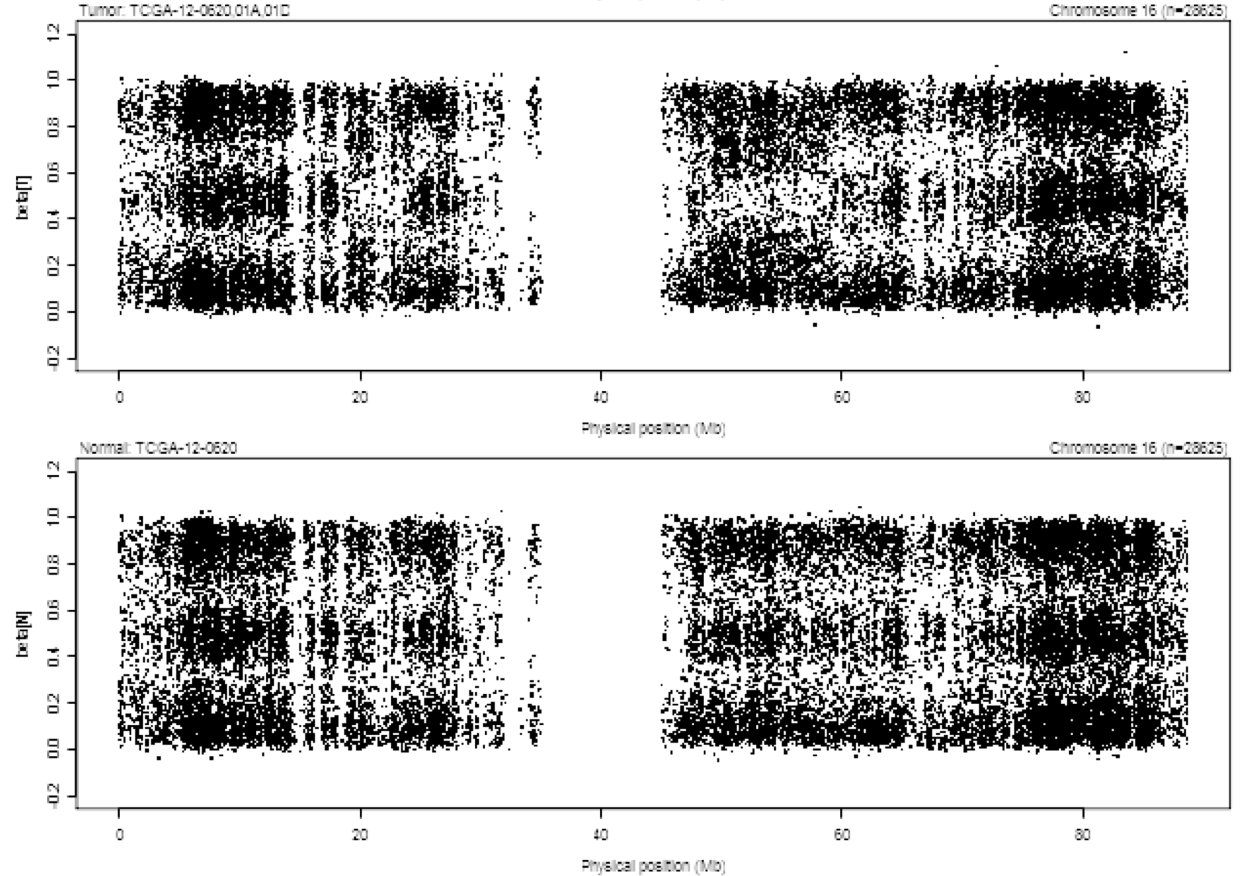
\includegraphics[height=5cm]{betaGenome}
  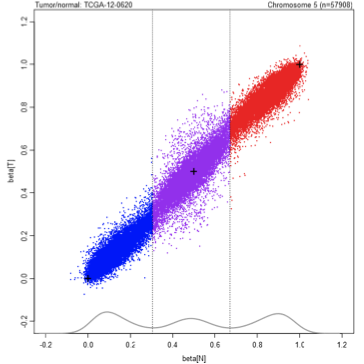
\includegraphics[height=5cm]{betaNVsBetaT}
}
%\caption{
\emph{Fraction of allele B $(\beta)$ in a tumor and its matched normal on chrosomosome XXX. Each point corresponds to a SNP. Left: $\beta$  along chromosome XXX for the tumor (top) and its matched normal (bottom). Right: Scatter plot of $\beta$ in the tumor vs $\beta$ in the normal. Black '+' indicate the location of normal genotype clusters: $(0,0)$, $(1/2,1/2)$ and $(1,1)$. Data were preprocessed using the CRMA~v2 method~\cite{BengtssonH_etal_2009b}.
}
%}

In figure XXX (right), most points are scattered along the diagonal but there is considerable deviation from the expected location of genotype clusters, even in the normal when no (or very few) genomic alterations are expected. Interestingly, this deviation is quite reproducible between the tumor and the normal. As a consequence of this deviation (left), genomic profiles of allele B fraction are quite noisy both in th tumor and the normal. 


\begin{PN}
  Shall we add a second illustration to illustrate the motivation for downstream analyses, ie  $(\theta_A,\theta_B)$ for a given sample across SNPs in a region as in Nancy's talk ?
\resizebox{0.96\columnwidth}{!}{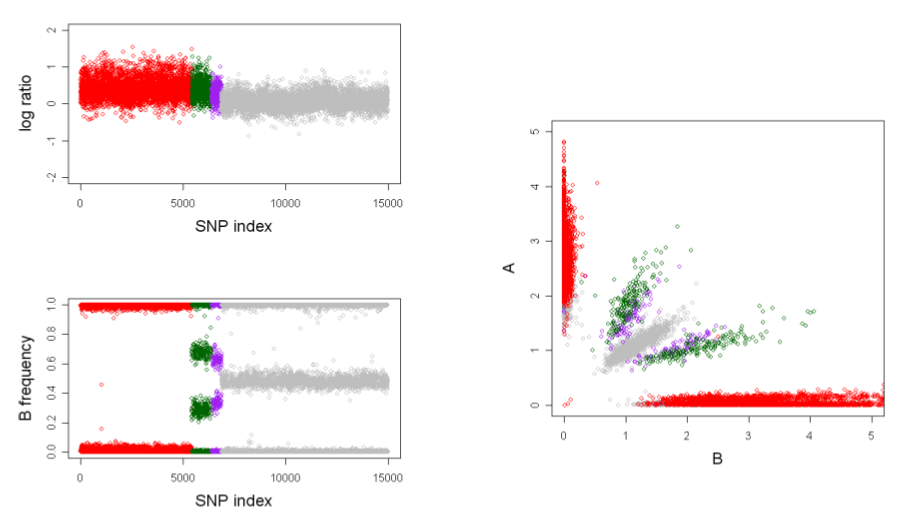
\includegraphics{thetaAcrossSNPs}}
\end{PN}

In this paper we present a method for calibrating the allele-specific copy-number estimates (ASCNs) of a tumor tissue given ASCNs of matched normal tissue or blood extract.  The method does not require external references and it is only the relative ASCNs that are calibrated, that is, the total CN estimates are not adjusted.



\subsection*{A single sample method}
The realization of a single-sample method has several implications:
(i) Each tumor-normal pair can be analyzed immediately without needing reference samples.
(ii) Samples can be processed in parallel on different hosts/processors making it possible to decrease the processing time of large data sets.
(iii) There is no need to reprocess a sample when new samples are produced, which further saves time and computational resources.
Furthermore, (iv) the decision to filter out poor samples can be made later, because a poor sample will not affect the processing of other samples.
More importantly, a single-sample method is
(v) more practical for applied medical diagnostics, because individual patients can be analyzed at once, even when they come singly rather than in batches.  This may otherwise be a limiting factor in projects with a larger number of samples.

The outline of this paper is as follows. 
In Methods, we describe the underlying model, how it is estimated, and an interpretation in terms of allelic crosstalk.
In Results, we show that the signal-to-noise ratios (SNRs) of the calibrated ASCNs are significantly larger than corresponding non-calibrated estimates.
In Discussion, we conclude the study, discuss potential limitations, ..., and give future research directions.


 
%%%%%%%%%%%%%%%%%%
\section*{Methods}
Let $(\theta_{N,j,A}, \theta_{N,j,B})$ be the signal intensities after preprocessing for SNP $j$ in the Normal (N) tissue, and $(\theta_{T,j,A}, \theta_{t,j,B})$ the corresponding intensitites in the tumor (T) tissue. The allele~B fraction~\cite{PeifferD_etal_2006} for SNP $j=1,\ldots,J$ in the nnormal ($N$) tissue is defined as:
\begin{equation}
  \beta_{N,j} = \frac{\theta_{N,j,A}}{\theta_{N,j}},
  \label{eqnCnLogRatio}
\end{equation}
where $\theta_{N,j} = \theta_{N,j,A} + \theta_{N,j,B}$ is the non-polymorphic signal at locus $j$.
\begin{PN}
do we really need index $j$ ? This is a SNP-specific model so we could probalby drop it.
\end{PN}

For a diploid SNP $j$, for which the genotype is either AA, AB or BB, we expect the allele~B fraction $\beta_{N,j}$ to be fall close to $0$, $1/2$, or $1$, respectively.
The allele~B fraction $\beta_{T,j}$ for the tumor ($T$) tissue/blood extract is defined analoguously. Because we cannot expected a SNP in a tumor to be diploid at any random SNP, we cannot make any prediction on where $\beta_{T,j}$ falls.

For a tumor-normal pair, we observe $(\beta_{N,j}, \beta_{T,j})$ at each SNP $j$.

\subsection*{Model and estimation}
Consider a SNP $j$ that is diploid in the normal tissue.  
Let the true genotype be denoted by the true allele~B fraction $\mu_{N,j}$ with possible states $\{0,1/2,1\}$ corresponding to genotypes $\{\gAA,\gAB,\gBB\}$.

Based on this, for SNP $j$ we model the observed allele~B fraction for the tumor and the normal pair as:
\begin{eqnarray}
  \beta_{T,j} = \mu_{T,j} + \delta_{j} + \eps_{T,j},\\
  \beta_{N,j} = \mu_{N,j} + \delta_{j} + \eps_{N,j},
  \label{eqnFracBModel}
\end{eqnarray}
where $\delta_{j}$ is a SNP-specific effect and $\eps_{T,j}$ and $\eps_{N,j}$ are independent zero-mean error terms. The difference $\mu_{T,j}-\mu_{N,j}$ can then be estimated straightforwardly from the data.
\begin{eqnarray}
  \widehat{\mu_{T,j}-\mu_{N,j}} = \beta_{T,j} - \beta_{N,j},
  \label{eqnTumorBoostEstimate}
\end{eqnarray}

% \begin{TODO}
%   Illustration: plot of $\beta_N$ vs $\beta_T$ (with lines with $y-x=c$ for $c \in$ seq(-1, 1, length=5), say) and tracks of $\beta_T$, $\beta_N$ and $\beta_T-\beta_N$. 
% \end{TODO}

\subsection*{Model interpretation in terms of allelic crosstalk}
\label{secACCModel}
In~\cite{BengtssonH_etal_2008} and \cite{BengtssonH_etal_2009b} it is argued that there exist crosstalk between the allele signals.  For instance, for a diploid SNP that is truly AA we will not only observe a great signal in the \PMA probes, but also some signal in the \PMB probes.  One explanation for this is crosshybridization due to the close similarity of probe sequences.  In the afformentioned studies, the authors propose an offset and crosstalk correction that is applied globally (to the six different heterozygous groups).  In addition, \cite{BengtssonH_etal_2009b} suggest to apply an additional nucleotide-position probe sequence normalization, which further corrects for imbalances between the two alleles.  It is shown that these corrections significantly improve the ability to detect total CN changes.
However, when looking at the distribution of the allele-specific summaries for a particular SNP $j$ across a set of samples, that is $\{(\theta_{ijA},\theta_{ijA})\}_i$, it is clear that for some SNPs there exists a remaining crosstalk, which is likely to be SNP specific.  In Figure~XXX, the allele-specific summaries for SNP\_A-XXXXXX in data set XXXXXX are shown, which clearly shows that the two homozygous genotype groups AA and BB are not located along the axes, that is, they are not orthogonal. For this particular SNP the heterozygote groups is located along the diagonal as expected.

\begin{TODO}
  Illustration: something like the following $(\theta_A,\theta_B)$ plots across samples for two or three consecutive SNPs (maybe with CNA, CNB instead to avoid the discussion about the copy number scale ?) Left: normal and tumor before calibration. Right: same with the calibrated tumor. Argue that the angle is really different from SNP to SNP. 
\resizebox{0.96\columnwidth}{!}{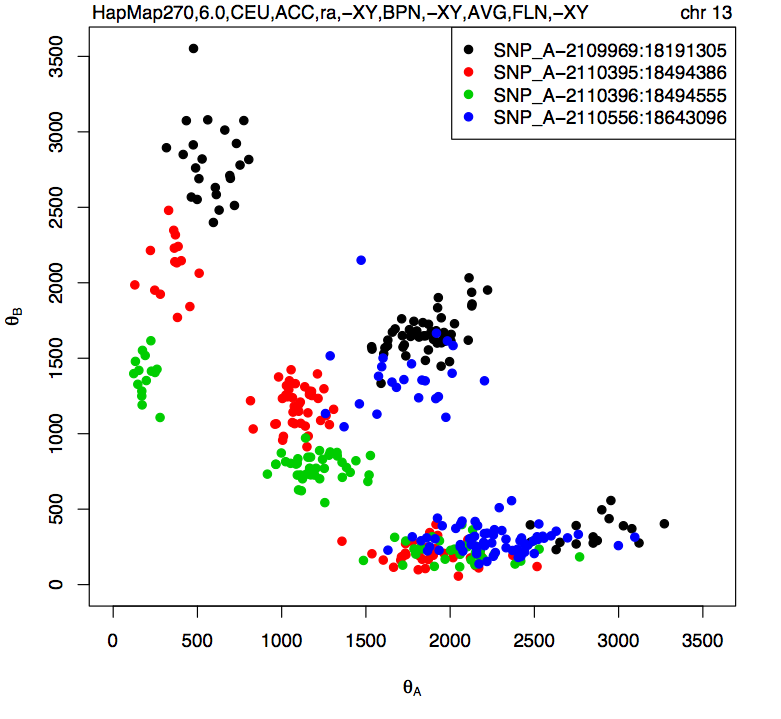
\includegraphics{thetaAcrossSamples} 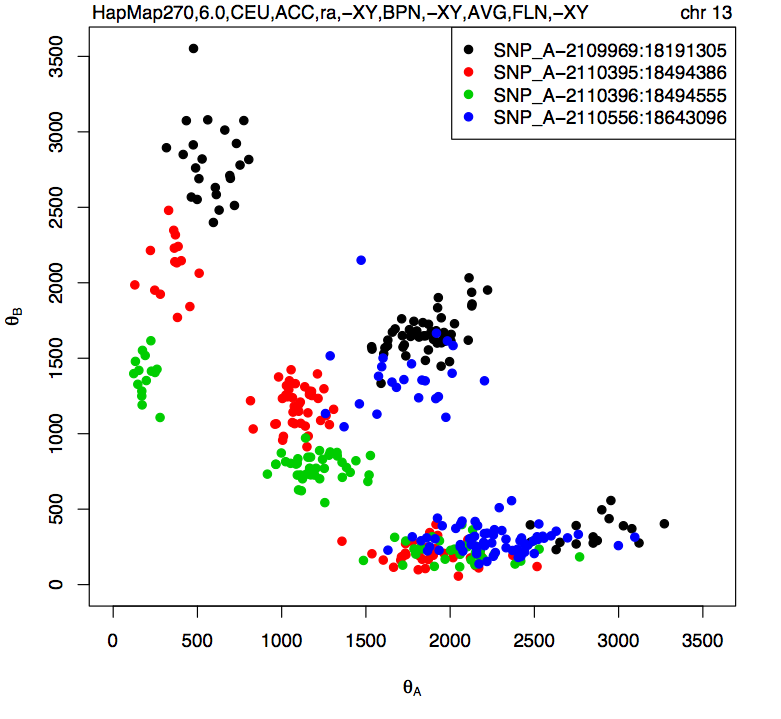
\includegraphics{thetaAcrossSamples}}
\end{TODO}


We propose the following crosstalk model for estimated allele-specific summaries $\{(\theta_{ijA},\theta_{ijA})\}_i$:
\begin{equation}
  \btheta_{ij} = \bS_i \bx_{ij} + \beps_{ij},
  \label{eqnACCi}
\end{equation}
where 
\begin{equation}
 \bS_i = 
 \begin{bmatrix}
   S_{iAA} & S_{iAB} \\
   S_{iBA} & S_{iBB}
 \end{bmatrix}
  \label{eqnACCii}
\end{equation}


%--------------------------------------------------------------------------
% EVALUATION METHODS
%--------------------------------------------------------------------------
\subsection*{Evaluation methods}
\label{secEvaluation}
cf CRMAv2. Given a region with a known alteration, considering that Hets are known, show that the two classesare better separated after calibration than before. Focus on copy neutral events that could not be detected from TCN\\

Show sensitivity to genotype calls by comparing results with naive genotyping, TGCA genotypes, and ``random'' genotypes.

%%%%%%%%%%%%%%%%%%%%%%%%%%%%
%% Results and Discussion %%
%%
\section*{Results}
\label{secResults}

%--------------------------------------------------------------------------
% DATA SET
%--------------------------------------------------------------------------
\subsection*{Data set}
We used data from the  Cancer Genome Atlas (TCGA) project~\cite{CollinsBarker_2007,TCGA_2008c}, a collaborative initiative to better understand cancer using existing large-scale whole-genome technologies.  Several tumor types are or are planned to be studied, including brain cancer (glioblastoma multiforme; GBM), ovarian cancer and lung cancer. 
 
From the Data Coordinating Center (\url{http://tcga-data.nci.nih.gov/tcga/homepage.htm}), we downloaded (Jan 2009) raw data (Level~1; CEL files) for a set of GBM tumor-normal pairs.
For the purpose of illustrating our method, we will focus mainly on sample TCGA-02-0104 (vials 01A vs 10A), because it has a large number of CN aberrations on Chr~3 at different mean levels.

\subsection*{Allele~B fraction before and after calibration}

\begin{PN}
  Add $(\theta_A, \theta_B)$ plots for each sample in a right panel (colored by region ?) and/or $(\beta_T^*, \beta_N)$ plots to each of the next 3 plots in order to get another sense of the improvement ?
\end{PN}

% \begin{figure}[!tpbh]
\begin{center}
\resizebox{0.96\columnwidth}{!}{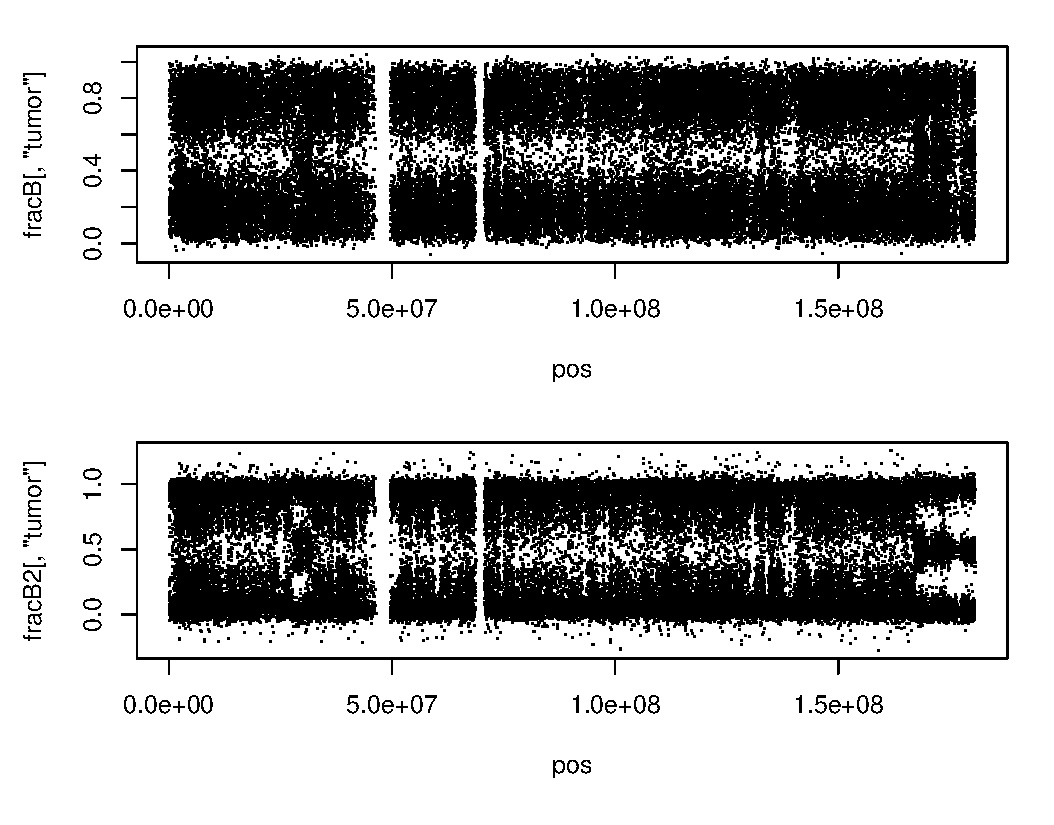
\includegraphics{TCGA-02-0069,tumor,Chr05,fracB,beforeAndAfter}}%
 \label{figROCs,chr05}
\end{center}
%  \caption{
%  }
% 
% \end{figure}

% \begin{figure}[!tpbh]
\begin{center}
  \resizebox{0.96\columnwidth}{!}{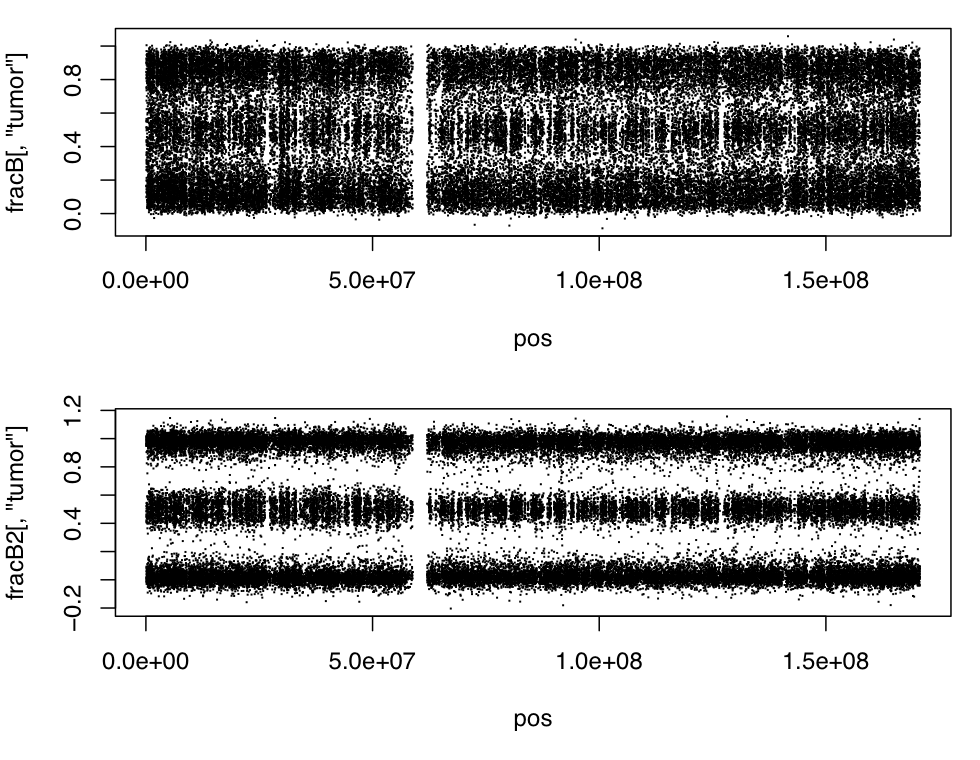
\includegraphics{TCGA-02-0069,tumor,Chr06,fracB,beforeAndAfter}}%
\label{figROCs,chr06}
\end{center}
%  \caption{
%  }
% \end{figure}


% \begin{figure}[!tpbh]
\begin{center}
  \resizebox{0.96\columnwidth}{!}{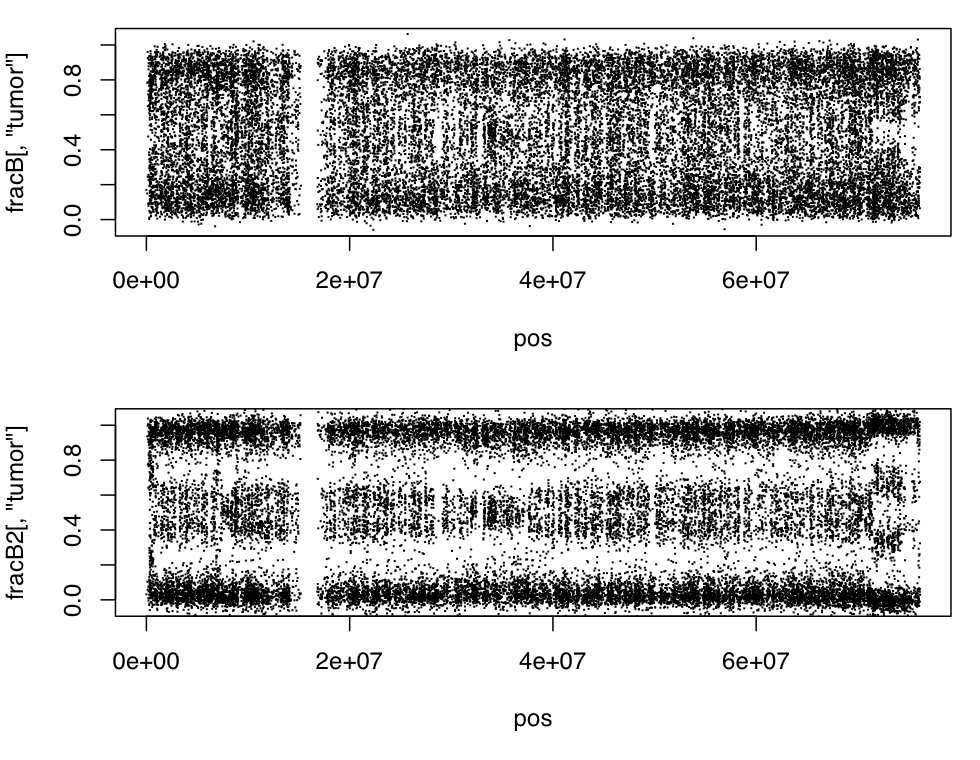
\includegraphics{TCGA-02-0069,tumor,Chr18,fracB,beforeAndAfter}}%
 \label{figROCs,chr18}
\end{center}
%  \caption{
%  }
% \end{figure}



\section*{Discussion}
\label{sec:discussion}

\subsection*{Downstream analysis methods}
= increasing power to detect copy number events, and making it possible to detect copy number neutral events from Affymetrix genotyping arrays, e.g.: 
\begin{itemize}
\item Segmentation of ASCN when normal genotypes are available
\item Iterative segmentation of ASCN when normal genotypes are not available
\item Quantile segmentation of ASCN when normal genotypes are not available
\end{itemize}

 When genotype calls for the normal sample are available they can be used to segment tumor ASCNs using any copy number segmentation algorithm. When these genotype calls are not avaiable we propose two algorithms that achieve joint segmentation of normal and tumor ASCNs, both leading to genotype calls for the normal sample as a by-product.\\

\subsection*{Genotyping errors}
In the Results section we have shown that our calibration methods leads to an improved signal ratio at the chromosome or at the genome scale. However the correction factor is genotype-specific, so if the normal genotype call for a given SNP is wrong, the correction factor will actually add bias to the estimated fraction of allele B. We argue that this is not a serious issue, for two main reasons:
\begin{itemize}
\item we can take genotype \emph{confidence scores} into account, either by discarding SNPs for which we are not confident in the genotype or by  using the confidence scores in whatever downstream analyses. 
\begin{TODO}
  in suppl. mat.: a section with beta along the genome after calibration for different levels of stringency for genotype calls (for the naive genotyping)
\end{TODO}
\item although our method does improve allele-specific copy number calls at the single locus level whenever normal genotype calls are correct, our goal is to improve the SNR of the fraction of allele B \emph{along the genome} in order to facilitate downstream analyses. In the results section we showed that our calibration method leads to a significant improvement of this SNR regardless of the genotype calling algorithm chosen. 
\end{itemize}

\subsection*{Extensions of the method}
\begin{itemize}
\item applicability / usefulness for Illumina data. paragraph on why Affy is more noisy than Illumina ? Sequences are all the same for Illumina, hence no probe sequence specific effects.
\item multi source version
\item multi sample (unpaired) version ?
\end{itemize}

    

%%%%%%%%%%%%%%%%%%%%%%
\section*{Conclusions}
  Text for this section \ldots


\section*{Algorithm and implementation}
The TumorBoost calibration method is available in R~\cite{RDevel_2008} package \pkg{aroma.cn} part of the \pkg{aroma.affymetrix} framework~\cite{BengtssonH_etal_2008b}.  The  method is designed and implemented to have bounded-memory usage, regardless of the number of samples/arrays processed. 
Furthermore, the complexity of the algorithm is linear in the number of loci ($J$).
Since it is a single-sample method, the tumor-normal pairs can be calibrated in parallel on multiple hosts/processors.
The method applies estimates obtained by SNP technology.




    
%%%%%%%%%%%%%%%%%%%%%%%%%%%%%%%%
\section*{Authors contributions}
    Text for this section \ldots

    

%%%%%%%%%%%%%%%%%%%%%%%%%%%
\section*{Acknowledgements}
  \ifthenelse{\boolean{publ}}{\small}{}

We gratefully acknowledge the TCGA Consortium and all its members for the TCGA Project initiative, for providing samples, tissues, data processing, and making data and results available.

\emph{Funding}: NCI grant U24 CA126551.

\emph{Conflict of interest}: none declared.

 
%%%%%%%%%%%%%%%%%%%%%%%%%%%%%%%%%%%%%%%%%%%%%%%%%%%%%%%%%%%%%
%%                  The Bibliography                       %%
%%                                                         %%              
%%  Bmc_article.bst  will be used to                       %%
%%  create a .BBL file for submission, which includes      %%
%%  XML structured for BMC.                                %%
%%                                                         %%
%%                                                         %%
%%  Note that the displayed Bibliography will not          %% 
%%  necessarily be rendered by Latex exactly as specified  %%
%%  in the online Instructions for Authors.                %% 
%%                                                         %%
%%%%%%%%%%%%%%%%%%%%%%%%%%%%%%%%%%%%%%%%%%%%%%%%%%%%%%%%%%%%%


{\ifthenelse{\boolean{publ}}{\footnotesize}{\small}

%  \bibliographystyle{bmc_article}  % Style BST file
%   \bibliography{bmc_article} }     % Bibliography file (usually '*.bib' ) 
\bibliographystyle{bmc_article}
\bibliography{bioinformatics-journals-abbr,hb-at-maths.lth.se}}
% \bibliography{hb-at-maths.lth.se}

%%%%%%%%%%%

\ifthenelse{\boolean{publ}}{\end{multicols}}{}



\end{bmcformat}
\end{document}




